% !TEX root = main.tex
\section{Performance Benchmarks}
\label{sec:performanceBenchmarks}

GraalVM bietet die Option statt des Graal-Compilers auch den HotSpot-Compiler zu nutzen. Dadurch kann mit verhältnismäßig wenig Aufwand
die Startzeit und der Speicherbedarf einer Anwendung, abhängig vom verwendeten Compiler verglichen werden. Bei einem trivialen Java-Microservice, implementiert in den populären
Microservice Frameworks Quarkus, Micronaut und Helidon\footnote{Diese Frameworks nutzen GraalVM standardmäßig als Anwendungsplattform}, konnten erhebliche Unterschiede bei der Startzeit und 
beim Speicherbedarf festgestellt werden, je nachdem welcher Compiler genutzt wurde. Wenn der Microservice mit dem Graal-Compiler zu einem \textit{native image} kompiliert wurde, war die Startzeit um
ca. den Faktor 50 schneller (siehe Abb. \ref{fig:system_startuptime}) und der Speicherbedarf um ca. den Faktor 5 geringer (siehe Abb. \ref{fig:system_memory_footprint}) war,
 als bei der Java HotSpot VM. Auch bezüglich der entgegengenommenen Anfragen pro Sekunde wurde mithilfe eines, in Quarkus implementierten
 trivialen REST-Services ein Vergleich durchgeführt. Nach der Warmup-Phase (ca. 70.000 Requests) liegen sowohl das \textit{native-image} als auch die HotSpotVM fast gleichauf mit ~31.000 Requests die pro
 Sekunde verarbeit werden können. Anzumerken hierbei ist allerdings, dass während der Warmup-Phase das \textit{native-image} wesentlich mehr Request pro Sekunde verarbeiten kann und schneller die
 Spitzenleistung erreicht (siehe Abb. \ref{fig:system_request}).
\begin{figure}[h]
	\centering
	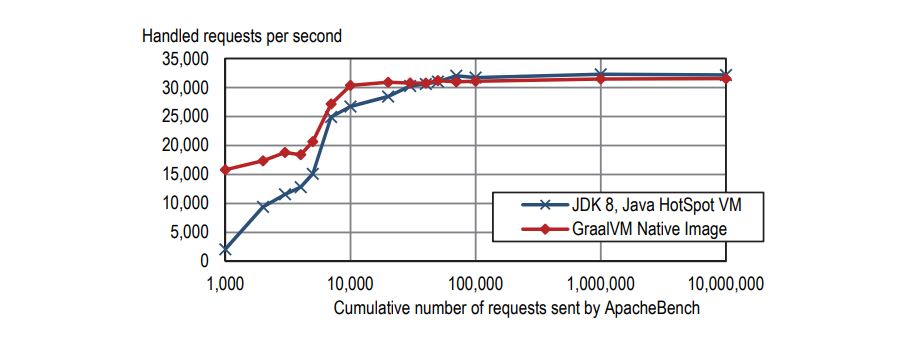
\includegraphics[width=.9\textwidth]{resources/requests_vergleich.png}
	\caption{Spitzenleistung von einem REST-basierten Service in Quarkus \parencite[Fig.12]{Wimmer2019}}
	\label{fig:system_request}
\end{figure} 
\newpage
\begin{figure}[h]
	\centering
	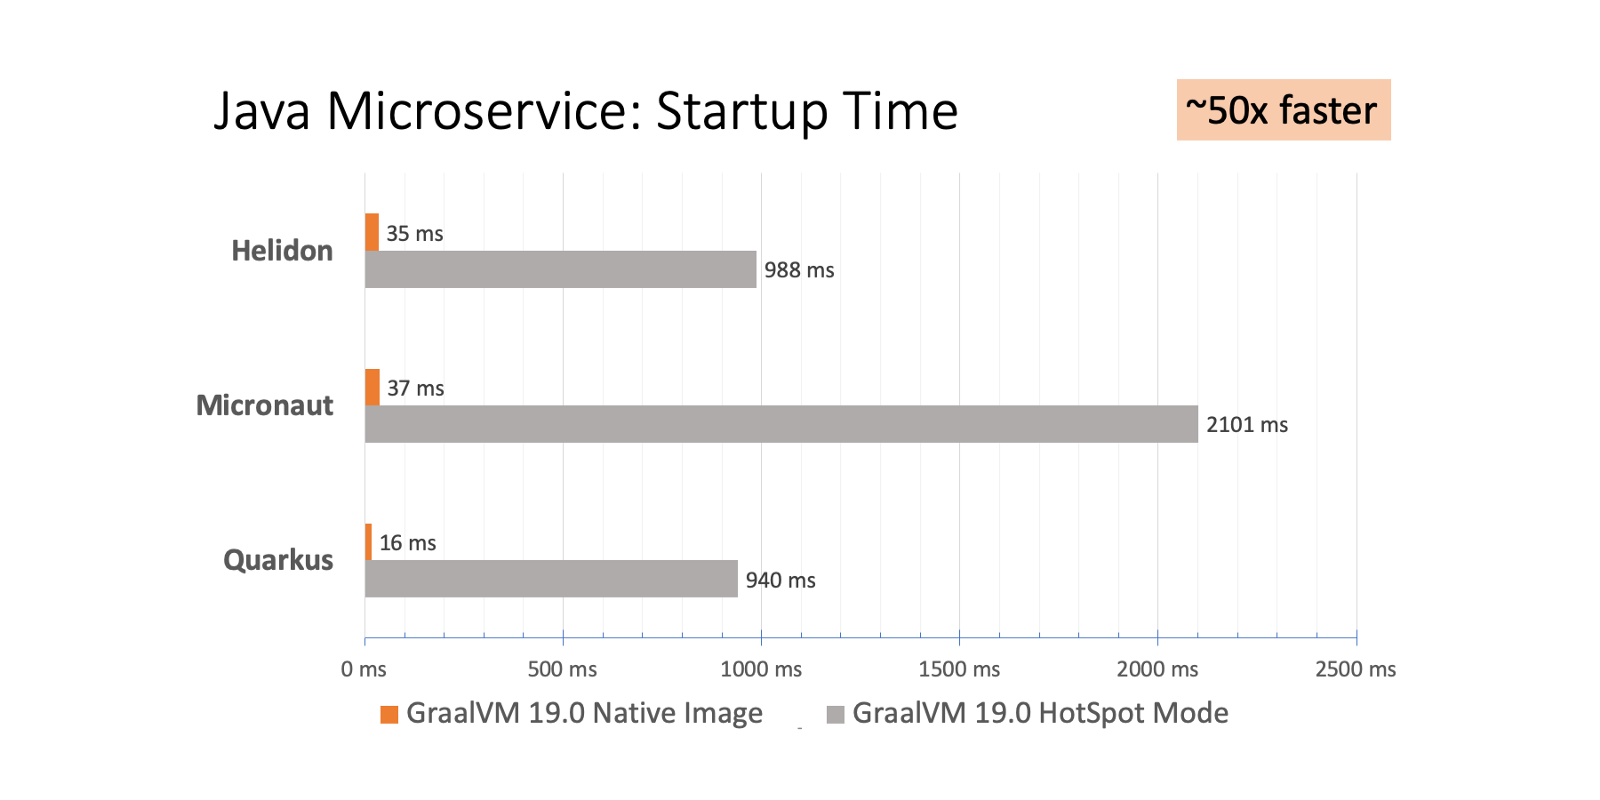
\includegraphics[width=.9\textwidth]{resources/ms_startup_time.png}
	\caption{Microservices Frameworks Startzeiten mit Native Image \parencite{GraalVMBenchmarks}}
	\label{fig:system_startuptime}
\end{figure}
\begin{figure}[h]
	\centering
	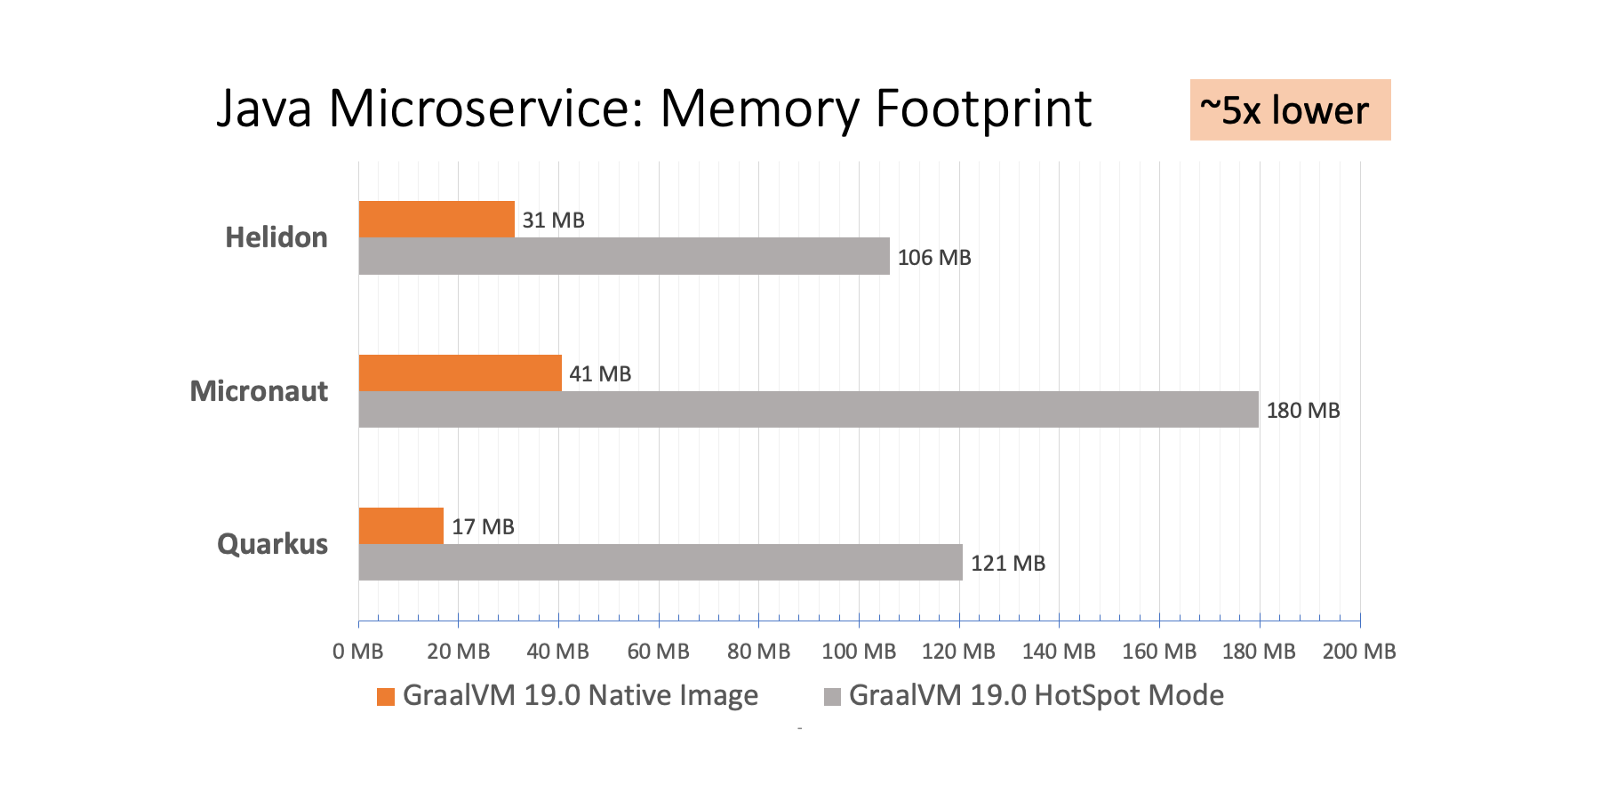
\includegraphics[width=.9\textwidth]{resources/ms_memory_footprint.png}
	\caption{Microservices Frameworks Speicherbedarf mit Native Image \parencite{GraalVMBenchmarks}}
	\label{fig:system_memory_footprint}
\end{figure}
